%!TEX program = xelatex

\documentclass[compress]{beamer}
%--------------------------------------------------------------------------
% Common packages
%--------------------------------------------------------------------------
\usepackage[english]{babel}
\usepackage{pgfpages} % required for notes on second screen
\usepackage{graphicx}
\usepackage{subfigure}
\usepackage{multicol}

\usepackage{tabularx,ragged2e}
\usepackage{booktabs}

\usepackage{setspace}

%--------------------------------------------------------------------------
% Load theme
%--------------------------------------------------------------------------
\usetheme{hri}

\usepackage{dtklogos} % must be loaded after theme
\usepackage{tikz}
\usetikzlibrary{calc,mindmap,backgrounds,positioning,svg.path}

\graphicspath{{figs/}}

\renewcommand{\bf}{\Medium}

%--------------------------------------------------------------------------
% General presentation settings
%--------------------------------------------------------------------------
\title{You’re Doing It Wrong!}
\subtitle{Studying Unexpected Behaviours in Child-Robot Interaction}
\date{ICSR 2015 -- Séverin Lemaignan, Julia Fink, Francesco Mondada,
Pierre Dillenbourg}
\author{\textit{Presented by} Alexis Jacq}
\institute{Computer-Human Interaction\\for Learning and Instruction {\Medium
EPFL}}

%--------------------------------------------------------------------------
% Notes settings
%--------------------------------------------------------------------------
%\setbeameroption{show notes on second screen}
%\setbeameroption{hide notes}

\begin{document}

\maketitle

%%%%%%%%%%%%%%%%%%%%%%%%%%%%%%%%%%%%%%%%%%%%%%%%%%%%%%%%%%%%%%%%%%%%%%%%%%%%%%%
%%%%%%%%%%%%%%%%%%%%%%%%%%%%%%%%%%%%%%%%%%%%%%%%%%%%%%%%%%%%%%%%%%%%%%%%%%%%%%%
%%%%%%%%%%%%%%%%%%%%%%%%%%%%%%%%%%%%%%%%%%%%%%%%%%%%%%%%%%%%%%%%%%%%%%%%%%%%%%%

\section{What happen when a robot does not obey?}

\begin{frame}{No, I don't want your tile!}
    \centering
    \video{0.8\textwidth}{videos/disobey.mp4}
\end{frame}

\begin{frame}{Two hypotheses}
\begin{enumerate}
    \item<1-> {\bf A robot that mis-behaves from time to time is more
        engaging}
    \item<2-> {\bf The way the robot ``mis-behaves'' betrays its cognitive
    capabilities}
\end{enumerate}

\only<3>{
If that's indeed the case, we gain an actionable technique to (1) sustain
engagement, (2) influence on cognitive attributions.
}

\end{frame}

%%%%%%%%%%%%%%%%%%%%%%%%%%%%%%%%%%%%%%%%%%%%%%%%%%%%%%%%%%%%%%%%%%%%%%%%%%%%%%%%%
\section{Unexpected behaviour, you said?}

\begin{frame}{Design of three behaviours}
\begin{enumerate}
    \item the robot get {\bf LOST}, for no visible reason;
    \item the robot {\bf DISOBEY};
    \item the robot makes a {\bf MISTAKE}.
\end{enumerate}
\end{frame}

\begin{frame}{LOST condition}
    \centering
    ...induces the perception of a \emph{contingent malfunction} \\
    (My robot has a {\bf bug}!)
    \par
    \includegraphics[width=0.6\textwidth]{domino-lost}
    \par
    \uncover<2>{
        {\bf Hypothesis}: decreased attribution of human-likeness
    }
\end{frame}

\begin{frame}{DISOBEY condition}
    \centering
    ...induces the perception of a robot's {\bf own will}
    \par
    \includegraphics[width=0.5\textheight]{domino-disobey}
    \par
    \uncover<2>{
        {\bf Hypothesis}: increased attribution of human-likeness
    }
\end{frame}

\begin{frame}{MISTAKE condition}
    \centering
    \only<1>{The robot goes wrong, but recognizes the error and repairs.}
    \only<2->{{\bf To err is human}. And the robot is aware of its own state (introspection)
    and of the expected state of interaction.}
    \par
    \includegraphics[width=0.5\textheight]{domino-mistake}
    \par
    \uncover<3>{
        {\bf Hypothesis}: increased attribution of human-likeness
    }
\end{frame}

\section{Experimental Procedure:\newline the Dominos task}

\begin{frame}{The Dominos task}
One child has to align the dominos, and at each turn, he/she ask for the next
one.

But the dominos are hidden in the room: the second child needs to find the
requested one, and give it to the robot (which is the only one allowed to cross
the dangerous river!)

\end{frame}

\begin{frame}{Correct behaviour}
    \only<1> {
    \centering
        \includegraphics[width=0.9\textwidth]{domino-setup}
    }
    \only<2> {
    \centering
        \video{0.8\textwidth}{videos/correct.mp4}
    }
    \only<3> {
        Note the non-verbal interaction cues:
        \begin{itemize}
            \item light patterns (yellow blink: ``Give me a domino!'', green pattern:
                ``I got it!'')
            \item sounds (different sounds for ``I got it!'' or ``Domino removed!'')
        \end{itemize}
    }
\end{frame}

\begin{frame}{LOST condition}
    \centering
    \only<1> {
        \includegraphics[width=0.9\textwidth]{domino-setup-lost}
    }
    \only<2> {
        \video{0.8\textwidth}{videos/lost.mp4}
    }

\end{frame}

\begin{frame}{DISOBEY condition}
        \centering
        \includegraphics[width=0.9\textwidth]{domino-setup-disobey}
\end{frame}

\begin{frame}{MISTAKE condition}

    \centering
    \only<1>{
        \includegraphics[width=0.9\textwidth]{domino-setup-mistake}
    }
    \only<2> {
        \video{0.8\textwidth}{videos/mistake.mp4}
    }
\end{frame}

\begin{frame}{The experiment}
    \begin{itemize}
        \item<1-> Wizard-of-Oz protocol;
        \item<2-> 13 pairs of children, 4-5 years old;
        \item<3-> Between subject: each pair sees one type of mis-behaviour;
        \item<4-> 14 turns per pair, alterning correct behaviours with
            mis-behaviours -- 14 min per group in average;
        \item<5-> Interactions video-recorded and annotated;
        \item<6-> Two interviews, in the middle of the experiment and at the
            end.
    \end{itemize}
\end{frame}

\section{Analysis}

\begin{frame}{Two dimensions}
    \begin{itemize}
        \item Analyse of the {\bf behaviour}: actions towards the robot,
            measured by annotating the videos;
        \item Analyse of the {\bf perception}: interviews.
    \end{itemize}
\end{frame}

\imageframe{interactions}

\begin{frame}{Behaviour towards the robot}

    Manual annotation of the video records:
    \begin{itemize}
        \item Touching the robot;
        \item Talking to the robot;
        \item Showing objects to the robot;
        \item Mis-using/mis-behaving with the robot;
        \item Looking at the experimenter (as a measure of ``what happen? what's
            wrong with the robot?'');
        \item Gesturing in front of the robot (waving the hand, etc.)
    \end{itemize}
\end{frame}


\begin{frame}{Results}
    \begin{center}
    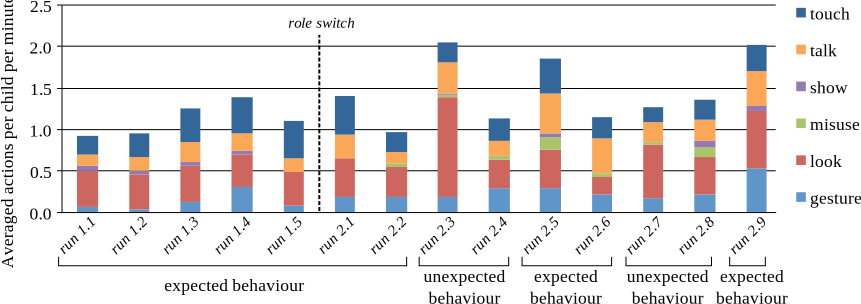
\includegraphics[width=\textwidth]{domino-time-active}
    \end{center}

    \only<2>{Significantly more actions toward the robot once the robot starts to
    mis-behave. This is expected.}

    \only<3>{No significant differences between conditions:\\ we do not measure
    a change of children's attitude with different kind of mis-behaviours.}

\end{frame}

\begin{frame}{Perception of the robot: Interviews}

    \begin{itemize}
        \item<1-> One interview after familiarization, but before introducing
            mis-behaviours;
        \item<2-> One interview at the end;
        \item<3-> Semi-structured, ``informal'' discussion (interviewing 4-5 years
            old is a challenge!).
    \end{itemize}

\end{frame}

\begin{frame}{Constructs and Questions}
\scriptsize
    \begin{multicols}{2}
    \begin{table}[]
        \begin{tabularx}{\linewidth}{p{0.9\linewidth}}

    \toprule
    {\bf Expectations} \tabularnewline
    \midrule
    \emph{How do you imagine a robot?} \tabularnewline
    \emph{What could it look like?} \tabularnewline
    \emph{Have you ever seen a robot before?} \tabularnewline

    %%
    \toprule
    {\bf Impression} \tabularnewline
    \midrule


    \emph{When you first saw R, what did you think?} \tabularnewline
    \emph{Is R a robot? How do you know?} \tabularnewline
    \emph{Did you expect R would come over to you when you call it?} \tabularnewline
    \emph{What happened when you put the domino in the box?} \tabularnewline

    %%
    \toprule
    {\bf Ascribe intention} \tabularnewline
    \midrule


    \emph{Do you think R could go out the door all by itself?} \tabularnewline	
    \emph{Does R always obey / come over to you?} \tabularnewline
    \emph{Could R do something silly?} \tabularnewline
    \emph{Why did R not come over to you when you called it?} \tabularnewline

            \bottomrule
        \end{tabularx}
        \label{tab:options}
    \end{table}

    \begin{table}[]
        \begin{tabularx}{\linewidth}{p{0.9\linewidth}}


    %%
    \toprule
    {\bf Ascribe perceptual capabilities} \tabularnewline
    \midrule


    \emph{Here is a domino. Do you think R can see it?} \tabularnewline 
    \emph{When I say \textit{``Hello R!''}, do you think R can hear it?} \tabularnewline

    %%
    \toprule
    {\bf Ascribe emotional state} \tabularnewline
    \midrule


    \emph{Does R have feelings? Can R be happy or sad sometimes?}
    \tabularnewline

    %%
    \toprule
    {\bf Social acceptance} \tabularnewline
    \midrule


    \emph{Do you like R? Why (not)?} \tabularnewline
    \emph{What do you (not) like about it?} \tabularnewline
    \emph{Would you like to have R at home?} \tabularnewline

    %%
    \toprule
    {\bf Companionship} \tabularnewline
    \midrule


    \emph{Could R be your friend? Why (not)?}\tabularnewline

    %%
    \toprule
    {\bf Ascribe moral standing} \tabularnewline
    \midrule


    \emph{Assume you go on a holiday for two weeks. Is it alright to leave R
    alone at home? Why (not)?} \tabularnewline


            \bottomrule
        \end{tabularx}
        \label{tab:options}
    \end{table}
    \end{multicols}

\end{frame}

\begin{frame}{Results}
    \begin{center}
    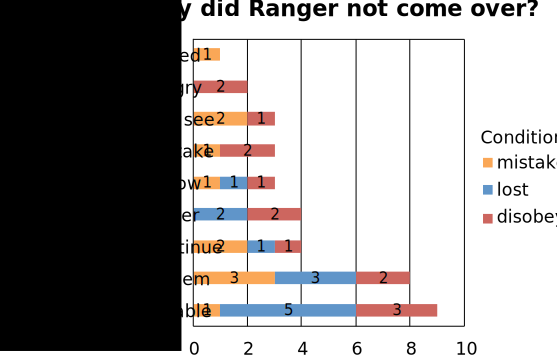
\includegraphics[height=0.6\textheight]{domino-why-misbehavior}
    \end{center}
\end{frame}


\begin{frame}{Results}
    \begin{center}
    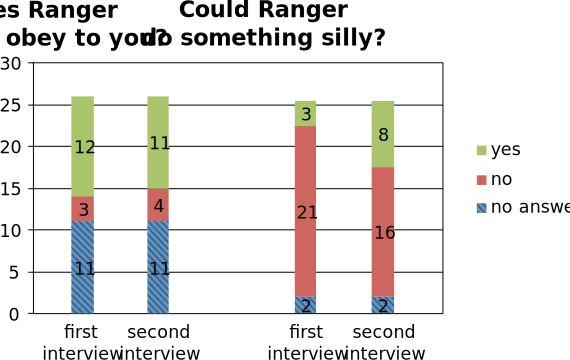
\includegraphics[height=0.6\textheight]{domino-intention}
    \end{center}
\end{frame}

\begin{frame}{Results}
    \begin{center}
    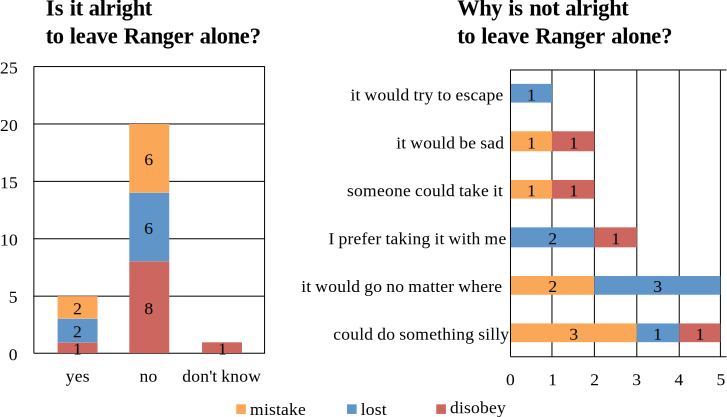
\includegraphics[height=0.6\textheight]{domino-leave-why}
    \end{center}
\end{frame}

\section{Compound anthropomorphism index?}

\begin{frame}{Index of anthropomorphism}
\end{frame}

\section{Take home message?}
\begin{frame}{Unexpected behaviours}
    \begin{tabular}{  >{\centering\arraybackslash}m{2cm} | >{\centering\arraybackslash}m{2cm} | >{\centering\arraybackslash}m{2cm} }
        & Unplanned by the robot & Planned by the robot \\ \hline
        Perceived as non-intentional & A  & B  \\ \hline
        Perceived as intentional &  C & D 
    \end{tabular}

\end{frame}

{
\fullbackground{ranger-background.jpg}
\begin{frame}{Anthropomorphism != Engagement}

\begin{figure}
    \hspace*{5cm}\includegraphics[width=0.6\textwidth]{domino-correlation}
\end{figure}
\end{frame}
}



{
\fullbackground{cheeky-ranger}
\begin{frame}[plain]

\setbeamercolor{hriSec1Demo}{fg=white}
\begin{beamercolorbox}[wd=\linewidth,ht=6ex,dp=0.7ex]{hriSec1Demo}
    \textbf{Thank you!}\\
    \scriptsize
    {\tt alexis.jacq@epfl.ch}\\
    {\tt severin.lemaignan@plymouth.ac.uk}
\end{beamercolorbox}
    \vfill

\end{frame}
}


\end{document}






